\documentclass{article}
\usepackage[utf8]{inputenc}
\usepackage[danish]{babel}

\usepackage{ragged2e}
\usepackage[labelfont=bf, font={small,it}]{caption}
\usepackage{graphicx}
\usepackage{float}
\usepackage[
    colorlinks=true,
    pdfborder={0 0 0},
    linkcolor=blue,
    citecolor=magenta
]{hyperref}

\graphicspath{ {images/} }

\title{Microservices og Availability}
\author{Adam Lass og Rasmus Helsgaun}
\date{11. december 2020}

\begin{document}

\maketitle
\begin{flushleft}
\subsection*{Abstract}

Ensuring high availability in a monolithic application is almost impossible due to its deployment challenges and lack of flexibility. This poses a big threat to businesses with a monolithic system today, that want to scale tomorrow. The solution to this problem is called microservices, and in this article we will explore why this is the architecture to use when building large systems with a lot of user traffic. By implementing microservices in the right places, businesses stand to win big on flexibility, scalability and availability of their systems.

\section*{Hvad indebærer availability?}

Når der er tale om availability, refereres der til tilgængeligheden af software og dets evne til at udføre en opgave når der er brug for det. Konceptet bygger på reliability, som handler om hvor pålidelig et system er, og inkorporerer tilmed også konceptet om gendannelse af systemet ved fejl. I denne artikel vil der blive set nærmere på hvordan en microservice arkitektur kan skabe værdi for en kunde i form af availability og hvilken bekostning har det sammenlignet med en monolitisk arkitektur.

\newpage
\section*{Hvad er en monolitisk arkitektur?}

Den monolitiske arkitektur beskriver en software applikation, hvor alle komponenter er samlet i et enkelt system. \linebreak

\begin{figure}[H]
    \captionsetup{justification=raggedright,singlelinecheck=false}
    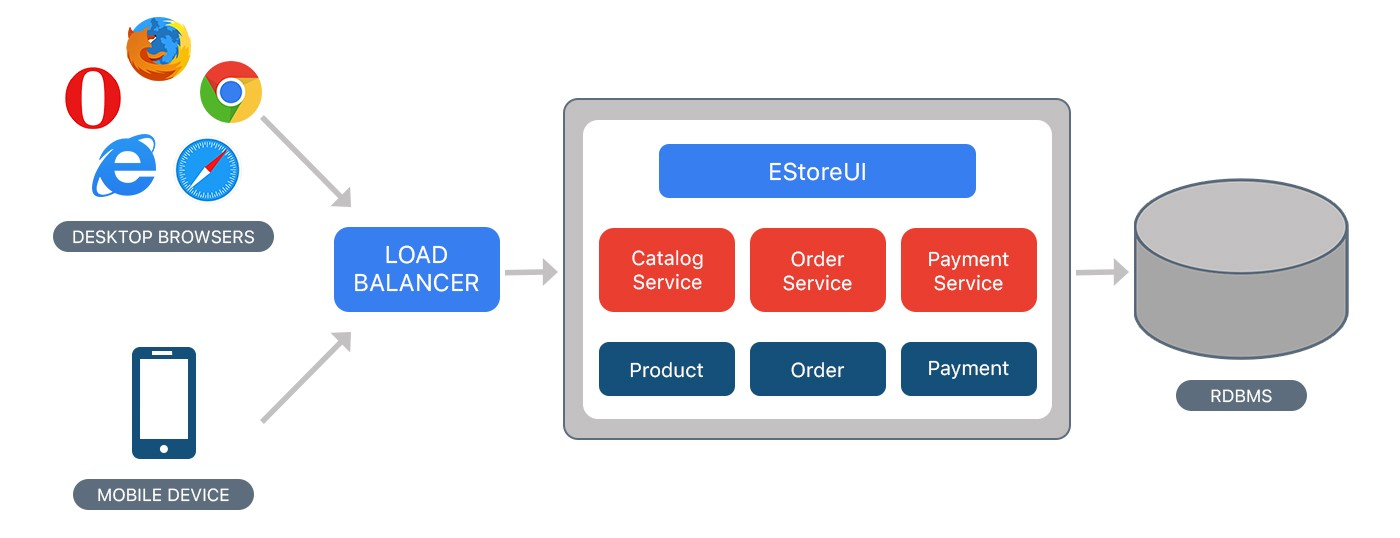
\includegraphics[width=\textwidth]{monolithic load balance.jpeg}
    \caption{Illustrerer opsætningen af den monolitiske arkitektur, med alle systemets komponenter samlet i ét modul bagved en load balancer.\cite{mono2} \label{figure:mono load balance}}
\end{figure}

Fordelene ved at bruge en monolitisk arkitektur er blandt andet, at det i de tidlige stadier kan være enkelt at udvikle, deploye og teste, da man har alle komponenter samlet i én applikation.\cite{mono1} Givet at ens monolitiske system er udviklet stateless, er det også forholdsvist simpelt at skalere horisontalt, ved at køre flere instanser af systemet bag en load balancer, som illustreret på figur 1.\cite{mono2} \linebreak

Der er dog også en række ulemper ved at udvikle og vedligeholde et monolitisk system, som bør overvejes inden den vælges som arkitektur. Eksempelvis kan det være sværere at vedligeholde et monolitisk system, da størrelsen af komponenterne og afhængighederne derimellem kan øge systemets kompleksitet. Den øgede kompleksitet medfører ofte en høj kobling, hvilket forværrer fleksibiliteten og overskueligheden af systemet.\cite{mono3} Dette kan have store negative implikationer for udefrakommende udvikleres forståelse og overblik af systemet, hvilket kan resultere i øgede tidsmæssige og økonomiske udgifter ved videreudvikling.\cite{mono4} \linebreak

Samtidigt kan størrelsen have betydning for en længere opstartstid, hvilket er essentielt at holde til et minimum under opdateringer eller efter at systemet er crashet. I sådanne tilfælde bærer arkitekturen i særdeleshed præg af at en lille opdatering eller crash af et komponent kræver et fuldt genstart af alle komponenterne.\cite{mono5} Hvis ikke disse scenarier bliver håndteret ordentligt, kan det resultere i at arkitekturen har en stor negativ indflydelse på reliability og availability af applikationen.

\section*{Hvad er Microservices?}

Microservices er applikationer som følger en arkitektur hvor deres formål er at specialisere sig i forskellige egenskaber, ofte som en del af et større system. Dette er et direkte modstykke til den monolitiske arkitektur, hvor man har alle egenskaber i samme system.\linebreak

\begin{figure}[H]
    \captionsetup{justification=raggedright,singlelinecheck=false}
    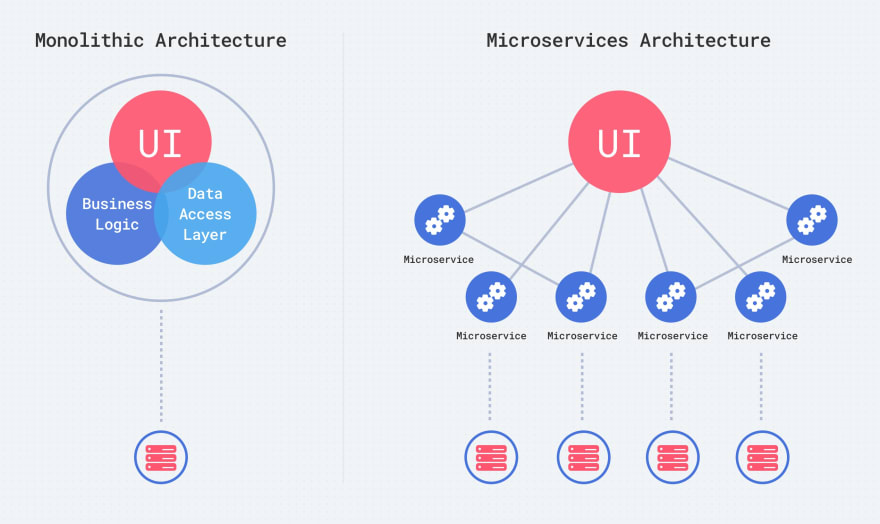
\includegraphics[width=\textwidth]{monolithic and microservices.jpg}
    \caption{Illustrerer forskellen mellem den Monolitiske arkitektur og Microservices arkitekturen.\cite{micro8}  \label{figure:mono micro}}
\end{figure}

Den opdelte arkitektur set i figur 2 bringer en række fordele til områder af udviklingen i form af availability, scalability, testability, deployment m.fl., men har selvfølgelig samtidigt også en række ulemper med sig.\cite{mono2} En meget dominerende fordel ift. availability er eksempelvis hvordan microservices gerne skal være små og afgrænset i forhold til deres egenskaber.\cite{micro1} Dette har nemlig den betydning at potentiel downtime på den enkelte service bliver mindre alvorlig, da den nu kun eksisterer som en mindre del af et større system. Sådan en downtime kan være forårsaget af bugs der får servicen til at crashe, men også af almindelige opdateringer af servicen, begge ting som er forventelige i dagligdagen. I forhold til continuous deployment kan microservices til med drage fordel af rullende opdateringer såsom Kubernetes’ Rolling Updates\cite{micro2}, og på denne måde helt undgå downtime forårsaget af opdateringer. Denne teknik udnytter i høj grad horisontal scaling, hvilket sørger for at flere instanser af samme service eksisterer ved siden af hinanden, så hvis den ene fejler kan en anden bare overtage. Dette forudsætter at man implementerer en loadbalancer der ligger foran disse horisontalt skalerede services, hvilket kan resultere i længere udviklings- og responstid. Dog tillader denne metode, sammen med et framework såsom serverless, at man dynamisk kan skalere de enkelte microservices eller funktioner efter behov, hvilket både øger availability og kan give økonomiske besparelser.\cite{micro3} \linebreak
En anden betydelig fordel som microservices bringer er dets testability. Selvstændigheden  og isolationen af komponenterne gør nemlig at de er nemmere at teste, da der findes de samme afhængigheder til andre komponenter sammenlignet med et monolitisk system.\cite{micro4} Accepterer man det faktum at tests skaber bedre kode, der sjældnere fejler\cite{micro5}, så kan man sige at bedre testability i overført betydning også skaber bedre availability og reliability.\linebreak

I det store hele kommer microservices altså med en masse fordele i forhold til availability, men der ligger selvfølgelig også en række udfordringer forbundet med at implementere arkitekturen. Udviklingsmæssigt skal man som udvikler ofte bruge meget tid på at hver enkelt komponent kan stå alene. Dette indebærer ofte ting som authentication, authorization, logging, osv., alle ting som man i et monolitisk system kun skal implementere én gang.\cite{micro6} En anden udfordring er at de forskellige komponenter ofte skal snakke med hinanden via protokoller såsom HTTP, hvilket tilføjer ekstra netværkstrafik og compute hos eventuelle loadbalancers. Dette kan både resultere i længere svartider og større regninger hos cloud leverandøren, begge ting man gerne vil forsøge at undgå, især som en mindre virksomhed.\cite{micro7}

\section*{Hvad vælger man?}
Store tech giganter såsom Amazon, Netflix og Spotify startede ud med en monolitisk arkitektur, men det ses dog at den generelle udvikling går mod at bruge microservices.\cite{mono3} Denne udvikling skyldes i høj grad at microservices er bedre egnet til at håndtere de udfordringer der kommer med at bygge store systemer som skal kunne håndtere meget brugertrafik. Dette kommer på en bekostning af ekstra udviklings- og responstid, men disse udgifter bliver nemt opvejet af de fordele der ligger i at bruge microservices såsom availability, scalability og maintainability. Den monolitiske arkitektur har dog stadig sine fordele ved mindre projekter hvor der ikke er store spikes i trafikken. Her er den nemlig hurtigere at udvikle og ofte billigere at hoste. Når der skal vælges mellem de to arkitekturer kommer det i sidste ende an på hvilke behov man har her og nu. Disse behov kan over tid ændre sig, dog vil de i de fleste tilfælde kun gå i en retningen mod at bruge microservices. Står man derfor i et valg mellem de to, og hælder mest til at bruge microservices, kan man lige så godt gøre det her og nu, i stedet for i morgen.\linebreak

\bibliographystyle{unsrt}
\bibliography{references}
\end{flushleft}
\end{document}
